\documentclass[11pt, a4paper]{article}   	% use "amsart" instead of "article" for AMSLaTeX format

\usepackage{geometry}
\usepackage[parfill]{parskip}    		% Activate to begin paragraphs with an empty line rather than an indent
\usepackage{graphicx}				% Use pdf, png, jpg, or eps with pdflatex; use eps in DVI mode
\usepackage[english, american]{babel}
\usepackage{csquotes}
\usepackage{xr} % Fross cross-referencing between multiple tex-files
\usepackage{caption} % Removes [:] in figure captions
\usepackage[utf8]{inputenc}
\usepackage{amssymb}
\usepackage{amsmath}
\usepackage{bm}
\usepackage{amsthm}
\usepackage{stmaryrd}
\usepackage{verbatim}
\usepackage{enumerate} % Pretty lists with (i),(ii)...
\usepackage{color}
\usepackage{ebproof}
\usepackage{tikz}
\usepackage[style=ieee, citestyle=numeric, backend=biber]{biblatex}
\DeclareLanguageMapping{american}{american-apa}
\addbibresource{reference.bib}


\def\name{Kjetil Midtgarden Golid}

\theoremstyle{plain}
\newtheorem{theorem}{Theorem}
\newtheorem{corollary}[theorem]{Corollary}
\newtheorem{lemma}[theorem]{Lemma}

\theoremstyle{definition}
\newtheorem{definition}{Definition}
\newtheorem{example}[theorem]{Example}

\newcommand{\lar}{\leftrightarrow}
\newcommand{\todo}[1]{\footnote{\textcolor{red}{TODO:} #1}}
\newcommand{\ol}[1]{\overline{#1}}

\usetikzlibrary{matrix}

\title{Master WIP}
\author{\name}
\date{\today}
\begin{document}
	\maketitle
  \section{Introduction}
  \label{sec:Introduction}
  % !TEX root= ../main.tex
\section{Paradoxes}
\label{sec:Paradoxes}
A theory in propositional logic is semantically \textit{inconsistent} if it has no model, i.e., there exists no variable assignment making all formulae in the theory true.
Consider the following example:
\begin{align}
  x \wedge \neg x
\end{align}
While a sentence like $\neg a \rightarrow b$ can be satisfied by, for instance, letting both $a$ and $b$ be true, no such assignment can be made for the statement above.
The statement is therefore inconsistent.

A paradox is usually informally defined as something along the lines of \textit{``a statement that can be neither true nor false''}.
We can immediately note one thing from this intuitive definition:
Since no paradoxes can be true, all paradoxes are, by definition, inconsistent.
It is however not the case that all inconsistent theories are paradoxes.
Just consider the inconsistent statement, $x \wedge \neg x$ again: this statement simply seems false, and not paradoxical.

A different view is that a paradox is a \textit{dialetheia}, a sentence that is \textit{both} true and false\cite{sep-dialetheism}. We will however not spend much time exploring these philosophical differences, as this is not a philosophical paper and it won't change much for our definitions.

The liar sentence is probably the most famous example of a paradox:
\begin{quote}
  ``This sentence is false.''
\end{quote}
If the statement is true, then the statement is false, but if the statement is false, then the statement is true.
It can thus neither be true nor false.
Note how the liar sentence is a statement about other statements (in this case itself).
In order to study these kinds of meta-statements, we need a way to reference other statements within a statement.
In propositional logic, we can do this by giving statements "names" in the form of adding fresh variables with equivalences to their correponding statements\todo{bad wording?}.
Consider the left statements below, together with their corresponding named statements on the right.
\begin{align}
  a               && x_1 \leftrightarrow a\\
  a \wedge \neg a && x_2 \leftrightarrow a \wedge \neg a\\
  a \vee \neg a   && x_3 \leftrightarrow a \vee \neg a
\end{align}
By performing this naming-operation on these statements, one is obviously changing their truth value.
Even though we have one consistent, one inconsistent and one tautological statement on the left, all the statements become consistent after they have been named.
This is because we in all the cases above can find a truth value for $x_i$ that matches the one of the corresponding statement.
This will not be the case for paradoxes, so our new named statements will be consistent if and only if they are not paradoxical.

Consider the liar sentence.  It can be written as a named statement in the following way:
\begin{align}
  x \leftrightarrow \neg x
\end{align}
This statement is obviously inconsistent, making it a paradox by our newly acquired definition.  The study of \textit{discourses} takes this formalization a step further.

  % !TEX root= ../main.tex
\externaldocument{../proofs/cnf_to_gnf}
\section{Graph Normal Form}
\label{sec:Graph Normal Form}
A propositional theory over a set of variables $\Sigma$ is in \textit{graph normal form (GNF)}\cite{apal-digraph} if all its formulae have the following form:
\begin{align}
  x \leftrightarrow \bigwedge_{y \in I_x} \neg y
\end{align}
where $I_x \subseteq \Sigma$ and such that every variable occurs exactly once on the left of $\leftrightarrow$ across all the formulae in the theory.

There is a simple translation from a theory in conjunctive normal form to an equisatisfiable theory in graph normal form (shown in Appendix~\ref{sec:Translating CNF to GNF}).
Since conjunctive normal form is expressively complete, we get that any propositional theory, including our labelled statements, has an equisatisfiable GNF theory.

This means that any discourse can be represented with a GNF theory such that the discourse is paradoxical if and only if the GNF theory is inconsistent.
This GNF representation of discourses is interesting to us because GNF theories have a tight correspondence to graphs.
This correspondence lets us not only decide the satisfiability of a discourse theory by looking at certain features in the corresponding graph, but the graph also provides us with the actual models of the discourse, if they exist.

In order to express this logic/graph correspondence, we first need to establish some graph terminology.

  % !TEX root= ../main.tex
\section{Graphs, Kernels and Solutions}
\label{sec:Graphs, Kernels and Solution}
A directed graph (digraph) is a pair \textbf{G} = $\langle G,N \rangle$ where $G$ is a set of vertices while $N \subseteq G \times G$ is a binary relation representing the edges in \textbf{G}.
We use the notation $N(x)$ to denote the set of all vertices that are targeted by edges originating in $x$ (successors of $x$).
Similarly, $N^-(x)$ denotes the set of all vertices with edges targeting $x$ (predecessors of $x$).
We define these two functions formally as follows:
\begin{align}
  N(x) := \{y \;|\; (x,y) \in N\}\\
  N^-(x) := \{ y \;|\; (y,x) \in N \}
\end{align}

A simple \textit{path} is a sequence of distinct vertices $x_1,x_2,\dots,x_n$ such that for any consecutive pair $x_i,x_{i+1}$ from the sequence, we have $(x_i, x_{i+1}) \in N$.
We say that two paths are \textit{disjoint} if they do not share any vertices (possibly with the exception of their initial nodes).

The functions $N$ and $N^-$ can be extended pointwise to sets in the following way:
\begin{align}
  N(X) = \bigcup_{x \in X} N(x)\\
  N^-(X) = \bigcup_{x \in X} N(x)
\end{align}

A kernel is a set of vertices $K \subseteq G$ such that:
\begin{align}
  G \setminus K = N^-(K)
\end{align}
The above equivalence can be split up into two inclusions to be more easily understood:

$G \setminus K \subseteq N^-(K)$, saying that each vertex outside the kernel has to have an edge into the kernel (K is absorbing).

$N^-(K) \subseteq G \setminus K$, saying that each edge targeting a vertex within the kernel has to come from outside, thus no two vertices in the kernel are connected by an edge (K is independent).

Kernels heve been of great interest over several decades, mainly within the fields of game theory and economics.
The concept was first defined and used by Neumann and Morgenstern in \cite{neumann}.
In a graph representing some sort of a turn-based game, where vertices are states and edges are transitions between states, one can often work out winning strategies whenever one finds a kernel in the graph.
Whenever one is outside of the kernel, one always has the possibility of moving inside the kernel (since the kernel is absorbing), while inside the kernel one \textit{has} to move out of it (since the kernel is independent).
If you are the player with the choice outside the kernel, you can control the game and choose to stabilize it by always moving into the kernel, forcing the opponent to move out again on the next turn.

Deciding the existence of kernels in finite graphs has been shown to be an NP-complete problem\cite{chvatal}.
This should not be surprising, since we are in the middle of showing the equivalence between this problem and the problem of finding satisying models of PL theories (SAT), which we know is NP-complete \footnote{We are concerned with SAT over infinitary formulae in this paper, not the finite version from computer science.}.

We will get the correspondence between satisfying models of a discourse theory and kernels in a graph through an alternative, equivalent kernel definition called a \textit{solution}.

Given a directed graph \textbf{G} = $\langle G,N \rangle$, an assignment $\alpha \in 2^G$ is a function mapping every vertex in the graph to either 0 or 1.
A \textbf{solution} is an assignment $\alpha$ such that for all $x \in G:$
\begin{align}
  \alpha(x) = 1 \iff \alpha(N(x)) = \{ 0 \}
\end{align}
This means that for any node $x$, if $x$ is assigned 1, then all its successors have to be assigned  0, and if $x$ is assigned 0, then there has to exist a node assigned 1 among its successors.
A consequence of this definition is that all sink nodes (nodes with no outgoing edges) in the graph have to be assigned 1, since it vacuously does not point to any node assigned 1.
We use the notation $sol(\mathbf{G})$ to denote the set of all solutions of the graph \textbf{G}.

  % !TEX root= ../main.tex
\section{Discourse Theories and Digraphs}
\label{sec:Discourse Theories and Digraphs}
As mentioned earlier, there is a close connection between (1) models of a discourse, (2) kernels of a graph and (3) solutions of a graph.
While we have the equivalence between (2) and (3), we will now look at two functions connecting (1) and (2).
This correspondence was shown by Roy T. Cook in \cite{cook}.
We get the following definitions from \cite{apal-digraph}

$\mathcal{T}:$ translating a digraph \textbf{G} into a corresponding theory $\mathcal{T}(\mathbf{G})$ such that $sol(\mathbf{G}) = mod(\mathcal{T}(G))$.

$\mathcal{G}:$ translating a theory $T$ into a corresponding digraph $\mathcal{G}(T)$ such that $mod(T) = sol(\mathcal{G}(T))$.

Given any digraph \textbf{G} we get the theory $\mathcal{T}(\mathbf{G})$ by taking, for each $x \in G$, the formula $x \leftrightarrow \bigwedge_{y \in N(x)} \neg y$ where $\bigwedge \emptyset = 1$.\\

\begin{example}\label{ex:3graphs}
  \[
    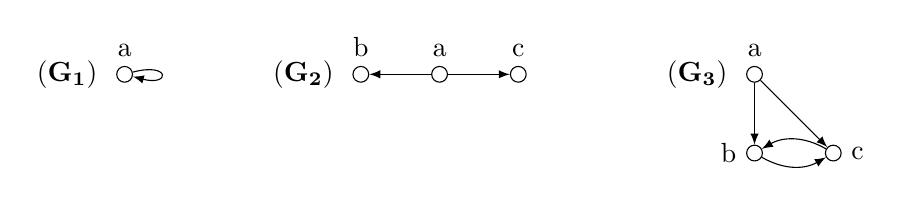
\begin{tikzpicture}
      [
      point/.style={circle,draw,inner sep=0pt,minimum size=2mm},
      collection/.style={thick,rectangle,draw,inner sep=0pt,minimum height=14mm, minimum width= 9mm}
      ]
      \node (label) at (0,1) [label=left:$(\mathbf{G_1})\;$] {};
      \node (0) at (0,1) [point,label=above:a] {};
      \draw [-latex, loop right] (0) to (0);

      \node (label) at (3,1) [label=left:$(\mathbf{G_2})\;$] {};
      \node (0) at (4,1) [point,label=above:a] {};
      \node (1) at (3,1) [point,label=above:b] {};
      \node (2) at (5,1) [point,label=above:c] {};
      \draw [-latex] (0) to (1);
      \draw [-latex] (0) to (2);

      \node (label) at (8,1) [label=left:$(\mathbf{G_3})\;$] {};
      \node (0) at (8,1) [point,label=above:a] {};
      \node (1) at (8,0) [point,label=left:b] {};
      \node (2) at (9,0) [point,label=right:c] {};
      \draw [-latex] (0) to (2);
      \draw [-latex] (0) to (1);
      \draw [-latex, bend right] (1) to (2);
      \draw [-latex, bend right] (2) to (1);
    \end{tikzpicture}
  \]
  Using the graphs from above, we get the following theories using $\mathcal{T}$:
  \begin{align}
    \mathcal{T}(\mathbf{G_1}) &= \big \{ a \leftrightarrow \neg a \big \} \\
    \mathcal{T}(\mathbf{G_2}) &= \big \{ a \leftrightarrow (\neg b \wedge \neg c), b, c \big \}\\
    \mathcal{T}(\mathbf{G_3}) &= \big \{ a \leftrightarrow (\neg b \wedge \neg c), b \leftrightarrow \neg c, c \leftrightarrow \neg b \big \}
  \end{align}

\end{example}
The fact that $sol(\mathbf{G}) = mod(\mathcal{T}(G))$ is shown in \cite{apal-digraph}.
Allthough not proving it, we can observe that $\mathbf{G_1}$ has no solution, just like its corresponding theory $\mathcal{T}(\mathbf{G_1})$ has no models.
$\mathbf{G_2}$ has one solution, where one assigns $a=0, b=1, c=1$.
This assignment also works as a model for $\mathcal{T}(\mathbf{G_2})$.
In $\mathbf{G_3}$, we get two solutions, both with $a$ assigned to 0, but with 0 and 1 distributed on $b$ and $c$.
These are also the only two models of $\mathcal{T}(\mathbf{G_3})$.

Conversely, given any discourse theory $T$ (in fact, this will work given any PL theory, since we can translate CNF to GNF), we can derive the corresponding graph $\mathcal{G}(T)$ in the following way:
All variables in the theory are vertices, and for each formula $x \leftrightarrow \bigwedge_{y \in I_x} y$ make a directed edge $\langle x,y \rangle$ for each $y \in I_x$.\\

\begin{example}
  \begin{align}
    ( a \lar \neg a'), (a' \lar \neg a), (b \lar \neg b'), (b' \lar \neg b), (y_1 \lar (\neg a \wedge \neg b \wedge \neg y_1))
  \end{align}
  Using $\mathcal{G}$ on the above GNF theory gives us the following graph:
  \[
    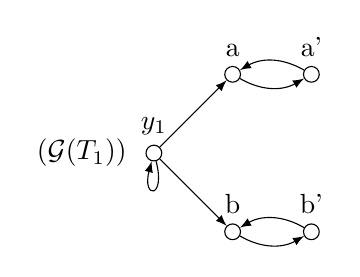
\begin{tikzpicture}
      [
      point/.style={circle,draw,inner sep=0pt,minimum size=2mm},
      collection/.style={thick,rectangle,draw,inner sep=0pt,minimum height=14mm, minimum width= 9mm}
      ]
      \node (label) at (5,1) [label=left:$(\mathcal{G}(T_1))\;$] {};
      \node (0) at (5,1) [point,label=above:$y_1$] {};
      \node (1) at (6,0) [point,label=above:b] {};
      \node (2) at (7,0) [point,label=above:b'] {};
      \node (3) at (6,2) [point,label=above:a] {};
      \node (4) at (7,2) [point,label=above:a'] {};
      \draw [-latex, loop below] (0) to (0);
      \draw [-latex] (0) to (1);
      \draw [-latex, bend right] (1) to (2);
      \draw [-latex, bend right] (2) to (1);
      \draw [-latex] (0) to (3);
      \draw [-latex, bend right] (3) to (4);
      \draw [-latex, bend right] (4) to (3);
    \end{tikzpicture}
  \]
\end{example}
Again, will we not be proving the correspondence, but notice that $T_1$ has one model satisfying it, where $a = 0$.
$\mathcal{G}(T_1)$ also has one solution, namely where $a = 0, a' = 1, y_1 = 0$.
$T_2$ has three solutions, where either $a$, $b$ or both are assigned $1$.
This reflects onto the graph since $y_1$ has to be assigned $0$, thus forcing $a$ or $b$ to be assigned $1$.
The fact that $\mathcal{G}$ gives us the correspondence we are looking for is shown in \cite{apal-digraph}.

This equivalence connects the fields of logic with the fields of graph theory:
With the problem of solutions in the graph being equivalent with SAT, we get our final equivalence between kernels in the graph and models of the theory.
A graph has a kernel if and only if its corresponding discourse is consistent (non-paradoxical).
A theory is paradoxical if and only if its corresponding graph has no kernels.
Because of this tight link, we will often refer to graphs without kernels as paradoxical graphs.

The applicability of kernels should by now be obvious.
In the next section we will review some of the various findings within Kernel Theory, and especially the findings related to infinitary graphs.

	% !TEX root= ../main.tex
\section{Results in Kernel Theory}
\label{sec:Results in Kernel Theory}
The end goal within Kernel Theory is ultimately to develop an easy way of answering the question ``Does this digraph have a kernel?'' no matter the graph, and no matter the answer.
As of today, we are not quite there, but a lot of work has been put into trying to identify special circumstances under which one is guaranteed to have (or guaranteed to not have) a kernel in the given graph.
One of the results is the Richardson's Theorem\cite{am-richardson}, worked out by Moses Richardson in 1953:\\

\begin{theorem}
  If D is a finitary\footnote{In a finitary graph, every vertex has a finite number of out-neighbors; the graph has finite branching.} digraph without odd cycles, then D has a kernel.
\end{theorem}

Intuitively, one might be tempted to believe that \textit{all} digraphs without odd cycles have kernels, but this is not the case.
Until now, our paradoxes have always been statements that -- directly or indirectly -- have been referring back to themselves (giving cycles in the graph) and thus causing a logical conflict, and it is hard to imagine any other way to construct paradoxical statements.
The following construction will however reveal our lack of imagination.

The \textit{Yablo Graph}\cite{analysis-yablo} is an example of an acyclic graph with no kernel.
It is constructed with an infinite set of vertices $\{ x_i | i \in \mathbb{N} \}$ and a set of edges $N$ such that $\langle x_i, x_j \rangle \in N$ iff $i < j$.
\[
  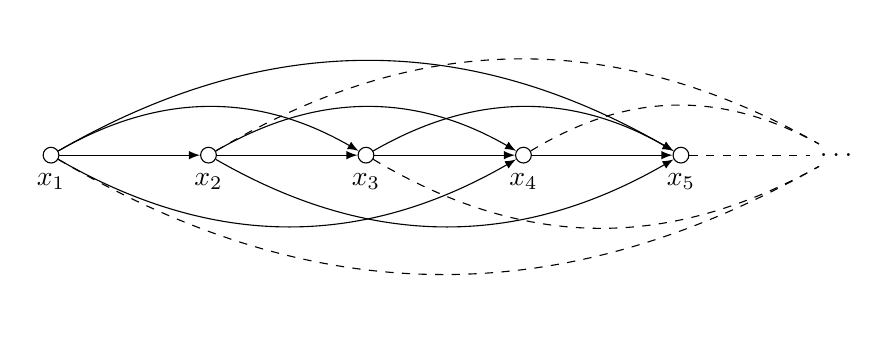
\begin{tikzpicture}
    [
    point/.style={circle,draw,inner sep=0pt,minimum size=2mm},
    collection/.style={thick,rectangle,draw,inner sep=0pt,minimum height=14mm, minimum width= 9mm}
    ]
    \node (1) at (0,1) [point,label=below:$x_1$] {};
    \node (2) at (2,1) [point,label=below:$x_2$] {};
    \node (3) at (4,1) [point,label=below:$x_3$] {};
    \node (4) at (6,1) [point,label=below:$x_4$] {};
    \node (5) at (8,1) [point,label=below:$x_5$] {};
    \node (6) at (10,1) [] {$\dots$};
    \draw [-latex] (1) to (2);
    \draw [-latex] (2) to (3);
    \draw [-latex] (3) to (4);
    \draw [-latex] (4) to (5);
    \draw [dashed] (5) to (6);
    \draw [-latex, bend left] (1) to (3);
    \draw [-latex, bend left] (2) to (4);
    \draw [-latex, bend left] (3) to (5);
    \draw [dashed, bend left] (4) to (6);
    \draw [-latex, bend right] (1) to (4);
    \draw [-latex, bend right] (2) to (5);
    \draw [dashed, bend right] (3) to (6);
    \draw [-latex, bend left] (1) to (5);
    \draw [dashed, bend left] (2) to (6);
    \draw [dashed, bend right] (1) to (6);
  \end{tikzpicture}
\]
Since there exist no two numbers $x,y \in \mathbb{N}$ such that $x < y$ and $y < x$, we get that the Yablo graph indeed is acyclic\todo{This is a bit over-simplified}.
Furthermore, since any natural number has infinitely many numbers strictly larger than it, we get that all the vertices are infinitely branching, making the Yablo graph infinitary (non-finitary).

The discourse represented by the Yablo graph would -- informally -- be the situation with an infinite number of statements, all saying ``Every statement after this statement is false''.

We will later show formally that the Yablo-graph is indeed without a kernel, but for now the following explanation will do.

Let us assume that the Yablo-graph \textit{has} a kernel and that the vertex $x_a$ is in it.
Then all the vertices to the right of $x_a$ are necessarily outside of the kernel, including $x_{a+1}$.
But if $x_{a+1}$ is outside of the kernel, it has to point to a vertex on the inside.
This is now impossible, since the out-neighborhood of $x_{a+1}$ is a subset of the out-neighborhood of $x_a$.
Since $x_a$ was chosen without any restrictions, no vertex can be inside the kernel, making it empty.
This is oviously not possible, so the Yablo-graph is without a kernel.

One thing should be mentioned at this point; neither odd cycles nor infinitely branching vertices \textit{entail} that their respective graphs are paradoxical.
The two following graphs illustrate this point:
\begin{align}
  \begin{aligned}
    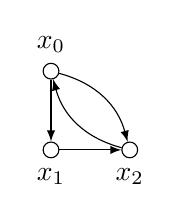
\begin{tikzpicture}
      [
      point/.style={circle,draw,inner sep=0pt,minimum size=2mm},
      collection/.style={thick,rectangle,draw,inner sep=0pt,minimum height=14mm, minimum width= 9mm}
      ]
      \node (0) at (0,1) [point,label=above:$x_0$] {};
      \node (1) at (0,0) [point,label=below:$x_1$] {};
      \node (2) at (1,0) [point,label=below:$x_2$] {};
      \draw [-latex] (0) to (1);
      \draw [-latex] (1) to (2);
      \draw [-latex, bend left] (2) to (0);
      \draw [-latex, bend left] (0) to (2);
    \end{tikzpicture}
  \end{aligned}
\end{align}
The above graph contains an odd cycle, but the singleton set $\{x_2\}$ is a kernel.
\begin{figure}[!h]
  \centering
  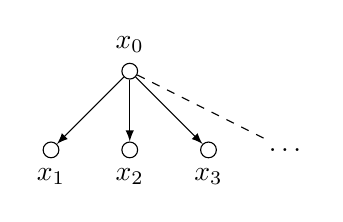
\begin{tikzpicture}
    [
    point/.style={circle,draw,inner sep=0pt,minimum size=2mm},
    collection/.style={thick,rectangle,draw,inner sep=0pt,minimum height=14mm, minimum width= 9mm}
    ]
    \node (0) at (1,2) [point,label=above:$x_0$] {};
    \node (1) at (0,1) [point,label=below:$x_1$] {};
    \node (2) at (1,1) [point,label=below:$x_2$] {};
    \node (3) at (2,1) [point,label=below:$x_3$] {};
    \node (4) at (3,1) [] {$\dots$};
    \draw [-latex] (0) to (1);
    \draw [-latex] (0) to (2);
    \draw [-latex] (0) to (3);
    \draw [dashed] (0) to (4);
  \end{tikzpicture}
  \caption{}
  \label{infinitary_with_kernel}
\end{figure}

The above graph has an infinitely branching vertex $x_0$, but the infinite set $\{x_i \;|\; x > 0\}$ is a kernel.

It is shown in \cite{apal-digraph} that every digraph (with at least one edge) can be transformed into a infinitary dag\footnote{Directed acyclic graph} such that $\alpha$ is a solution to the created dag if and only if it is a solution to the original digraph.
This means that for any finitary graph that is paradoxical by the virtue of having an odd cycle, there is an infinitary, \textit{acyclic} digraph that is also paradoxical.
So, if one is trying to find ways to identify paradoxical graphs, one does only need to look at dags.

This result will be of great importance to us, enabling us to narrow our search space when looking for paradoxes.

	% !TEX root= ../main.tex
\externaldocument{kernelthoery}
\section{Recognizing dags without kernels}
\label{sec:Recognizing dags without kernels}
Knowing that any graph can be translated to an equisatisfiable dag, the challenge is now to find sufficient conditions for dags to have kernels, even weaker than the one proved by Richardson (the fact that any finitary dag has a kernel is a direct consequence of Richardson's Theorem).

Michał Walicki has proposed the following thesis:
\begin{quote}
  ``If a dag has no kernel then it has a ray with infinitely many vertices dominating it.''
\end{quote}
Some terminology (given a graph $\mathbf{G} = \langle G,N \rangle$):
A \textit{ray} is an semi-infinite path, i.e. an infintie sequence $(x_1, x_2, \dots)$ of distinct vertices of $G$ such that $(x_i,x_{i+1}) \in N$ for each $i$.

A vertex $x_0$ \textit{dominates} a set of vertices $Y \subseteq G$ if there exists an infinite number of disjoint paths from $x_0$ to distinct vertices of $Y$.

The contrapositive of Walicki's thesis suggests a weaker condition for a kernel, since a dag having a ray with infinitely many vertices dominating it implies that the dag is infinitary.

	% !TEX root= ../main.tex
\externaldocument{discoursegraphs}
\externaldocument{kerneltheory}
\section{Resolving GNF-theories}
\label{sec:Resolving GNF-theories}
In this section, we present an inference system introduced by Walicki in \cite{michal-completeness} which handles clausal theories induced from GNF-theories.

Recall that a theory written in GNF has formulae of the following form:
\begin{align}
  x \lar \bigwedge_{i \in I_x} \neg y_i
\end{align}
Using simple operations only, one can manipulate these formulae into an equivalent set of clauses.
We start by writing the above bi-implication as two implications:
\begin{align}
  x \rightarrow \bigwedge_{i \in I_x} \neg y_i \quad\quad \text{and} \quad\quad x \leftarrow \bigwedge_{i \in I_x} \neg y_i
\end{align}
The first implication can be rewritten in the following way:
\begin{align}
  x \rightarrow \bigwedge_{i \in I_x} \neg y_i
  \quad\Leftrightarrow\quad \neg x \vee \bigwedge_{i \in I_x} \neg y_i
  \quad\Leftrightarrow\quad \bigwedge_{i \in I_x} (\neg x \vee \neg y_i)
  \quad\Leftrightarrow\quad \bigwedge_{i \in I_x} \neg (x \wedge y_i)
\end{align}
The second implication can be rewritten in the following way:
\begin{align}
  x \leftarrow \bigwedge_{i \in I_x} \neg y_i
  \quad\Leftrightarrow\quad x \vee \neg \left( \bigwedge_{i \in I_x} \neg y_i \right)
  \quad\Leftrightarrow\quad x \vee \bigvee_{i \in I_x} y_i
\end{align}
By splitting the conjunction from the first implication up into individual clauses, we get the following two kinds of clauses for every variable $x$ in the GNF theory:
\begin{align}
  \text{OR-clause:}&\quad x \vee \bigvee_{i \in I_x} y_i\\
  \text{NAND-clauses:}&\quad \neg (x \wedge y_i)\text{, for every }i \in I_x
\end{align}
We will treat both the OR-clauses and the NAND-clauses as sets of atoms, denoting NAND-clauses $\neg (x \wedge y)$ as $\overline{xy}$ and OR-clauses $x \vee y_1 \vee y_2 \vee y_3$ as $xy_1y_2y_3$.
This enables us to state things like $\overline{xy} \subset \overline{xyz}$.
A theory will -- as expected -- be a set of OR- and NAND-clauses.

If we interpret the initial GNF-theory as a graph $\mathbf{G}=\langle G,N\rangle$, for every vertex $x \in G$, there will be one OR-clause $\{ x \} \cup N(x)$ and for every edge $\langle x,y \rangle \in N$ there will be a NAND-clause $\overline{xy}$.
The graphs from Example~\ref{ex:3graphs} will have the following clausal theories:
\begin{align}
  \mathcal{T}(\mathbf{G_1}) &= \{ a, \ol{a} \}\\
  \mathcal{T}(\mathbf{G_2}) &= \{ abc, b, c, \ol{ab}, \ol{ac} \}\\
  \mathcal{T}(\mathbf{G_3}) &= \{ abc, bc, \ol{ab}, \ol{bc} \}
\end{align}
Further notation: $A\subseteq G$ denotes an OR-clause while $\ol{A} \subseteq G$ denotes a NAND-clause.
Given a graph $\mathbf{G}=\langle G,N\rangle$, we denote the set of all NAND-clauses induced from the graph as NAND and all induced OR-clauses as OR.
The combined set $\Gamma = NAND + OR$ will be our initial clauses in the inference system.
\subsection{The inference system}
\label{sub:The inference system}
We consider the following inference system, but we will focus mainly on proofs using the Axioms together with the (Rneg) rule.
\begin{align}
  \text{(Ax)} &\quad \Gamma \vdash C, \quad \text{for } C \in \Gamma\\
  \text{(Rneg)} &\quad \frac{ \{ \Gamma \vdash \ol{a_iA_i} \; |\; i \in I \} \quad \Gamma \vdash \{ a_i \; |\; i \in I \} }{ \Gamma \vdash \ol{\bigcup_{i \in I} A_i} }\\
  \text{(Rpos)} &\quad \frac{ \Gamma \vdash A \quad \{\Gamma \vdash B_iK_i \; |\; i \in I \} \quad \{ \Gamma \vdash \ol{a_ik} \; |\; i \in I, k \in K_i \} }{ \Gamma \vdash (A \setminus \{ a_i \; |\; i \in I \} ) \cup \bigcup_{i \in I} B_i }
\end{align}
(Rneg) is creating NAND-clauses from NAND-clauses using OR as a side-condition.
(Rpos) is creating OR-clauses from OR-clauses using NAND as a side-condition.
In (Rneg), $\ol{a_iA_i}$ denotes the NAND $\ol{\{ a_i \} \cup A_i}$ with a potentially empty $A_i$.

The premise of the (Rneg) rule is a set of $I$ NAND-clauses together with one OR-clause with $I$ elements such that each atom $a_i$ in the OR-clause is contained within a NAND-clause, and such that each NAND-clause contains an atom from the OR-clause.
The correspondence between the NAND-clauses and the elements of the OR-clause should in other words be bijective.
The conclusion is the union of all the NAND-clauses without their corresponding atom from the OR-clause.

Here are some examples of incorrect applications of the (Rneg)-rules, followed by some correct applications:
\begin{align}
  (1)\;\;\frac{\ol{ax}\quad\ol{by}\quad\ol{cz}}{\ol{xyz}}abx\quad\quad
  (3)\;\;\frac{\ol{ax}\quad\ol{by}}{\ol{xy}}abx\quad\quad
  (2)\;\;\frac{\ol{ax}\quad\ol{by}\quad\ol{bz}}{\ol{xyz}}abx
\end{align}
(1) is incorrect because the NAND $\ol{cz}$ contains no atoms from the OR $abx$.
(2) is incorrect because the number of NAND-clauses does not match the length of the OR-clause.
(3) is incorrect because there exist no bijective correspondence of the type described above.
\begin{align}
  (4)\;\;\frac{\ol{ax}\quad\ol{by}\quad\ol{cz}}{\ol{xyz}}abc\quad\quad
  (5)\;\;\frac{\ol{ax}\quad\ol{b}}{\ol{x}}ab\quad\quad
  (6)\;\;\frac{\ol{ax}\quad\ol{by}\quad\ol{xyz}}{\ol{xyz}}abx
\end{align}
The three above applications are all correct, since all the atoms in each OR-clause get matched to exactly one NAND-clause in such a way that no NAND-clause stays unmatched.

We set no restrictions on the number and cardinality of our clauses, meaning that there might be an infinite number of clauses, and both the OR-clauses and the NAND-clauses might be either finite or infinite in size.
Note that an infinite graph gives infinitely many NAND-clauses, while an infinitary graph also gives us infinitely long OR-clauses.

We study the refutation system that arises from the Axioms and the (Rneg)-rule, calling it Neg.
It is shown in \cite{michal-completeness} that Neg is sound and refutationally complete for theories with only a countable number of OR-clauses.
Soundness gives us that proving $\ol{C}$ for any $C \subseteq G$ implies that the vertices in $C$ cannot all be assigned 1 in the graph model.
Refutational completeness gives us that whenever a graph/theory is inconsistent, we are able to prove $\varnothing$ in Neg.

Note that Neg is not complete.
The following inconsistent graph exemplifies this:\par
\begin{figure}[!h]
  \centering
  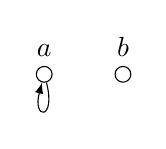
\begin{tikzpicture}
    [
    point/.style={circle,draw,inner sep=0pt,minimum size=2mm}
    ]
    \node (1) at (0,0) [point, label=above:$a$] {};
    \node (2) at (1,0) [point, label=above:$b$] {};
    \draw [-latex, loop below] (1) to (1);
  \end{tikzpicture}
  \caption{}
  \label{fig:neg_not_complete}
\end{figure}
Bacause of the loop on vertex $a$, the graph has no solutions.
We therefore have $\vDash \ol{b}$, but we are unable to prove $\ol{b}$ in Neg.
\subsection{Inconsistency of the Yablo-graph}
\label{sub:Inconsistency of the Yablo-graph}
The inconsistency of the Yablo-graph is easily proven using Neg only.
Since every vertex $x_i$ (using the notation from Figure~\ref{fig:yablo-graph}) has an edge to each vertex $x_j$ where $j > i$, we get that every pair of distinct vertices is connected by an edge.
This means that our set of axioms from the Yablo-graph looks like this:
\begin{align}
  \text{NAND} = \{ \ol{x_ix_j} \; |\; i < j\}
  \quad\quad\quad
  \text{OR} = \{ x_ix_{i+1}x_{i+2}\dots \; |\; i \in \mathbb{N}\}
\end{align}
For any vertex $x_i$ from the Yablo-graph, we are now able to prove $\ol{x_i}$ in the following way:
\begin{prooftree*}
  \Hypo{\ol{x_ix_{i+1}}}
  \Hypo{\ol{x_ix_{i+2}}}
  \Hypo{\ol{x_ix_{i+3}}}
  \Hypo{\dots}
  \Infer4[$x_ix_{i+1}x_{i+2}\dots$]{\ol{x_i}}
\end{prooftree*}
Proving $\varnothing$ is now simple:
\begin{prooftree*}
  \Hypo{\dots}
  \Infer1{\ol{x_1}}
  \Hypo{\dots}
  \Infer1{\ol{x_2}}
  \Hypo{\dots}
  \Infer1{\ol{x_3}}
  \Hypo{\dots}
  \Infer4[$x_1x_2x_3\dots$]{\varnothing}
\end{prooftree*}
A less trivial inconsistency proof is the one on the \textit{Stretched Yablo-graph}.
This proof can be found in the appendix together with the definition of Stretched Yablo.

It is worth mentioning that even though our focus has been -- and will be -- on theories originating from graphs, the results on soundness and completeness holds for any theory consisting of a set of NANDs and a set of ORs.

An example of this is the pigeonhole problem which easily can be represented as a set of NAND- and OR-clauses, but does not directly correspond to a graph (it can of course be translated to a graph theory, like any other propositional theory).
Proofs in Neg of pigeonhole problems of different size are to be found in the appendix\todo{some reference system needed}.

	% !TEX root= ../main.tex
\section{Thesis overview}
\label{sec:Thesis overview}
The soundness and refutational completeness of Neg makes it a potentially great tool in the overarching endeavor of weakening the conditions for kernels in graphs.
We know that for any graph $G$, $\varnothing$ can be proven in Neg based on $G$ if and only if $G$ is without a kernel.

Suppose that any inconsistency can be proven using only NAND-clauses of length at most 2, and that all NAND-clauses of length 2 corresponds to vertices related in a certain way in the graph.
This would in combination give us a condition for kernels, namely the absence of such specifically related vertices.
With this in mind, the thesis will set out to do two things:

(1) Define a graph structural relation such that two vertices $a,b$ in a graph $G$ are related if and only if $G \vdash \ol{ab}$.

This will be covered in Chapter 2 where we will be looking at increasingly general graph structures that ensures the provability of certain NAND-clauses, ultimately attempting to reach a structure general enough so that the provability of a NAND-clause entails the existence of that structure.

(2) Explore whether Neg is still refutationally complete when restricted to using NAND-clauses of length 1 or 2 only.

It will be shown in Chapter 3 that this is \textit{not} possible.
The chapter will present graphs where certain NAND-clauses are provable in general, but not under the restrictions mentioned.
This will then be used to show that the restrictions makes Neg unable to prove inconsistencies in certain graphs.

	\pagebreak
  \section{Proofs}
  \label{sub:Proofs}
  % !TEX root= ../main.tex
\section{Translating CNF to GNF}
\label{sec:Translating CNF to GNF}
Since any PL theory can be expressed in CNF, showing that any theory $P$ in CNF can be translated to a theory $R$ in GNF such that $P$ and $R$ are equisatisfiable gives us that any PL theory has an equisatisfiable GNF.

Given any CNF theory $P$, for each formula in it, follow the steps below to acquire its corresponding GNF theory.

\textbf{Step 1:}
For each literal $\neg x_i$ in the formula, introduce a fresh variable $x'_i$ and add the following two GNF formulae to $P$:
$x'_i \lar \neg x_i, x_i \lar \neg x'_i,$ (unless this has already been done while translating an earlier formula in the theory).

\textbf{Step 2:}
In each clause of the formula, replace every negative literal $\neg x_i$ with its corresponding $x'_i$ fom step 1.
Every clause in the formula does now contain positive literals only.

\textbf{Step 3:}
For every clause $(x_1 \vee x_2 \vee \dots \vee x_n)$, replace it with the following formula, where $y$ is fresh:
\[y \lar (\neg x_1 \wedge \neg x_2 \wedge \dots \wedge \neg x_n \wedge \neg y)\]

This formula is equisatisfiable with our original clause.

The combined set of all these acquired formulae will make up our GNF-theory.
We have only added proper GNF formulae and all variables appear to the left in exactly one clause, so $R$ will indeed be a GNF theory.

Step 1 is adding a bi-implication formula that is always satisfiable, since one of two variables in it is fresh.
One can think of it as a labelling of an already existing variable.
Thus, adding these formulae to a theory does not change its satisfiability/non-satisfiability.

Step 2 is replacing each negative literal with its label, also not changing the satisfiability.

Step 3 is replacing one formula with an equisatisfiable formula, thus not changing the overall satisfiability.

Since none of the steps above change the satisfiability of the theory, we can conclude that our acquired theory is equisatisfiable with to original CNF theory.

Below are some examples of CNF-theories with their corresponding GNF-theories.\\

\begin{example}
  \begin{align}
    \text{CNF:\quad}& ( a \vee b )\\
    \text{GNF:\quad}& ( a \lar \neg a'), (a' \lar \neg a), (b \lar \neg b'), (b' \lar \neg b), (y_1 \lar (\neg a \wedge \neg b \wedge \neg y_1))\\
    \\
    \text{CNF:\quad}& (\neg a)\\
    \text{GNF:\quad}& ( a \lar \neg a'), (a' \lar \neg a), (y_1 \lar (\neg a' \wedge \neg y_1))\\
  \end{align}
\end{example}

	\pagebreak
	% !TEX root= ../main.tex
\subsection{Inconsistency of Stretched Yablo}
\label{sub:Inconsistency of Stretched Yablo}

One variation of the Yablo-graph is the Stretched Yablo-graph, presented by Walicki in \cite{michal-completeness}.
While the Yablo-graph is a ray where each vertex on it has direct edges to all the vertices after it, the Stretched Yablo-graph is a ray where each vertex has \textit{disjoint paths} (with certain properties depending on the variation of Stretched Yablo) to all vertices in after it.

The variation on which we will be proving an inconsistency is one with a set of core vertices $\mathbb{N}$ where each vertex $x$ has a disjoint path to every vertex $y$ after it, such that the length of the path is $(2 \times (y - x) - 1)$.

\begin{figure}[!h]
  \centering
  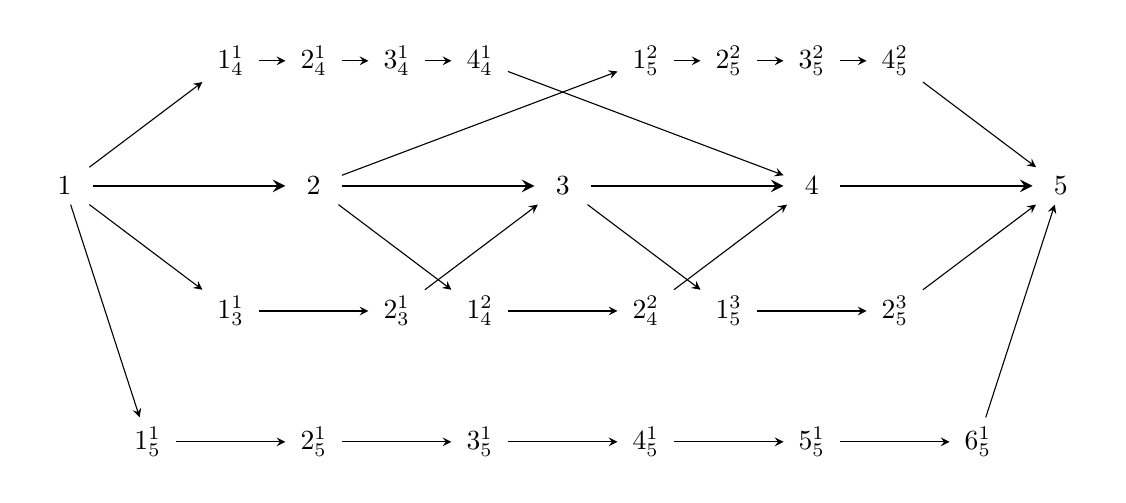
\begin{tikzpicture}
    [
    point/.style={circle,draw,inner sep=0pt,minimum size=2mm},
    collection/.style={thick,rectangle,draw,inner sep=0pt,minimum height=14mm, minimum width= 9mm}
    ]
	  \matrix (m) [matrix of math nodes,row sep=3em,column sep=1em,minimum width=2em]
	  {   & & 1^1_4 & 2^1_4 & 3^1_4 & 4^1_4 & & 1^2_5 & 2^2_5 & 3^2_5 & 4^2_5 & & \\
	  	1 & & & 2 & & & 3 & & & 4 & & & 5 \\
	  	  & & 1^1_3 & & 2^1_3 & 1^2_4 & & 2^2_4 & 1^3_5 & & 2^3_5 & & \\
		  & 1^1_5 & & 2^1_5 & & 3^1_5 & & 4^1_5 & & 5^1_5 & & 6^1_5 & \\
		};
	  \path[-stealth]
	  	(m-1-3) edge (m-1-4)
		(m-1-4) edge (m-1-5)
		(m-1-5) edge (m-1-6)
		(m-1-6) edge (m-2-10)
		(m-1-8) edge (m-1-9)
		(m-1-9) edge (m-1-10)
		(m-1-10) edge (m-1-11)
		(m-1-11) edge (m-2-13)
	  	(m-2-1) edge [line width=1pt] (m-2-4)
				edge (m-3-3)
				edge (m-1-3)
				edge (m-4-2)
		(m-2-4) edge [line width=1pt] (m-2-7)
				edge (m-3-6)
				edge (m-1-8)
		(m-2-7) edge [line width=1pt] (m-2-10)
				edge (m-3-9)
		(m-2-10) edge [line width=1pt] (m-2-13)
		(m-3-3) edge (m-3-5)
		(m-3-5) edge (m-2-7)
		(m-3-6) edge (m-3-8)
		(m-3-8) edge (m-2-10)
		(m-3-9) edge (m-3-11)
		(m-3-11) edge (m-2-13)
		(m-4-2) edge (m-4-4)
		(m-4-4) edge (m-4-6)
		(m-4-6) edge (m-4-8)
		(m-4-8) edge (m-4-10)
		(m-4-10) edge (m-4-12)
		(m-4-12) edge (m-2-13)
	  ;
	\end{tikzpicture}
  \caption{Stretched Yablo}
  \label{fig:stretched_yablo}
\end{figure}
Shown above are parts of the Stretched Yablo-graph described.
We denote the core vertices by natural numbers.
The peripheral vertices contained in each path is denoted by $n^x_y$ where $x$ and $y$ is the source and target, respectively, of the path in which the vertex is contained.
$n$ denoted the relative position on the path.

Based on the given definition of Stretched Yablo and the notation from above, we get the following sets of axioms:
\begin{align}
  N1a &= \{\; \ol{x(x+1)} \;&&|\; x \in \mathbb{N} \; \} \\
	N1b &= \{\; \ol{x1^x_y} \;&&|\; x,y \in \mathbb{N}, x+1 < y \; \} \\
	N2 &= \{\; \ol{n^x_y(n+1)^x_y} \;&&|\; n,x,y \in \mathbb{N}, x+1 < y, n < 2(y-x) - 2 \; \} \\
	N3 &= \{\; \ol{(2(y-x)-1)^x_yy} \;&&|\; n,x,y \in \mathbb{N}, x+1 < y \; \} \\
	O1 &= \{\; x(x+1)1^x_{x+2}1^x_{x+3}\dots \;&&|\; x \in \mathbb{N} \; \} \\
  O2 &= \{\; n^x_y(n+1)^x_y \;&&|\; n,x,y \in \mathbb{N}, x+1 < y, n < 2(y-x) - 2 \; \} \\
	O3 &= \{\; (2(y-x)-1)^x_yy \;&&|\; n,x,y \in \mathbb{N}, x+1 < y \; \}
\end{align}
We get that NAND = $N1a \cup N1b \cup N2 \cup N3$ and that OR = $O1 \cup O2 \cup O3$.
One can identify the different axioms by looking at the figure above\footnote{recall how NANDs corresponds to edges, while ORs corresponds to vertices}:
$N1a$ are the edges making up the core ray of the graph, $N1b$ are the edges going from a core vertex onto a peripheral vertex, $N2$ are the edges between two peripheral vertices and $N3$ are the edges going from a peripheral vertex back onto a core vertex.
$O1$ are the vertices on the core ray, $O2$ and $O3$ are the peripheral vertices, $O3$ being the ones that points back to a core vertex.

In order to prove $\varnothing$ from these axiom, we prove some intermediate clauses.

	\pagebreak
	\printbibliography
\end{document}
